% This is a general template file for the LaTeX package SVJour3
% for Springer journals. Original by Springer Heidelberg, 2010/09/16
%
% Use it as the basis for your article. Delete % signs as needed.
%
% This template includes a few options for different layouts and
% content for various journals. Please consult a previous issue of
% your journal as needed.
%
\RequirePackage{fix-cm}
%
%\documentclass{svjour3}                     % onecolumn (standard format)
%\documentclass[smallcondensed]{svjour3}     % onecolumn (ditto)
\documentclass[smallextended]{svjour3}       % onecolumn (second format)
%\documentclass[twocolumn]{svjour3}          % twocolumn
%
\smartqed  % flush right qed marks, e.g. at end of proof
%
\usepackage{graphicx}
\usepackage{authblk}
%
% insert here the call for the packages your document requires
%\usepackage{mathptmx}      % use Times fonts if available on your TeX system
%\usepackage{latexsym}
% etc.
\usepackage{mathptmx}      % use Times fonts if available on your TeX system
\usepackage{latexsym}% 
\usepackage{lineno}% 
\usepackage{amsmath}%
\usepackage{upgreek} % 
\usepackage{mathtools} % 
\usepackage{graphicx}% 
%\usepackage{subcaption}
\usepackage{tikz}% <<<<<<<<<<<< Added by Sadegh
%\linenumbers*[1]% <<<<<<<<<<<< Added by Sadegh
\usepackage{makecell}% <<<<<<<<<<<< Added by Sadegh
\usepackage{natbib}% <<<<<<<<<<<< Added by Sadegh
\usepackage{geometry}% <<<<<<<<<<<< Added by Sadegh
\usepackage{float}
\usepackage{subfigure}
\usepackage{caption}
\usepackage{subcaption}
\usepackage{booktabs}
\usepackage{multicol, blindtext}
\usepackage{arydshln}
\usepackage{wrapfig}
\floatstyle{plaintop}
\restylefloat{table}
% please place your own definitions here and don't use \def but
% \newcommand{}{}
%
% Insert the name of "your journal" with
% \journalname{myjournal}
%
\begin{document}

\title{Inter-comparison study of UT1-UTC from Intensives and 24-hour sessions for CONT17 campaign
%\thanks{}
}
% Grants or other notes about the article that should go on the front
% page should be placed within the \thanks{} command in the title
% (and the %-sign in front of \thanks{} should be deleted)
%
% General acknowledgments should be placed at the end of the article.

% \subtitle{Do you have a subtitle?\\ If so, write it here}

%\titlerunning{Short form of title}        % if too long for running head

\author{Shrishail Raut\textsuperscript{1,2}       \and
        Robert Heinkelmann\textsuperscript{1}     \and
        Sadegh Modiri\textsuperscript{1,2}           \and
        Kyriakos Balidakis\textsuperscript{1}          \and
         Santiago Belda\textsuperscript{3,4}                \and
         Harald Schuh\textsuperscript{1,2}
}

\authorrunning{Shrishail Raut et al}
\institute{Shrishail Subhash Raut \and Robert Heinkelmann \and Sadegh Modiri \and Kyriakos Balidakis \and Harald Schuh \at
             GFZ German Research Centre for Geosciences, Potsdam, Germany \\
             Technische Universit{\"a}t Berlin, Institute for Geodesy and Geoinformation Science, Berlin, Germany
           \and
          Santiago Belda \at
             Image Processing Laboratory (IPL) - Laboratory of Earth Observation (LEO), University of Valencia, Valencia, Spain
             \\
             UAVAC, University of Alicante, Alicante, Spain
              \and
              \textsuperscript{1} GFZ German Research Centre for Geosciences, Potsdam, Germany  \\
              \textsuperscript{2} Technische Universit{\"a}t Berlin, Institute for Geodesy and Geoinformation Science, Berlin, Germany \\ 
              \textsuperscript{3} Image Processing Laboratory (IPL) - Laboratory of Earth Observation (LEO), University of Valencia, Valencia, Spain\\
              \textsuperscript{4}  UAVAC, University of Alicante, Alicante, Spain
}

\date{Received: date / Accepted: date}
% The correct dates will be entered by the editor

\maketitle

\begin{abstract}
This work deals with validating the established approach of analyzing VLBI intensive sessions to determine dUT1. VLBI sessions from the CONT17 campaign are chosen as they provide continuous VLBI observations over two weeks (28th Nov - 12th Dec 2017) of the currently highest quality. For the standard 24-hour sessions in this campaign, two different legacy networks were involved, the IVS network, which was entirely based on IVS network stations with global distribution, and VLBA network involving VLBA and a few IVS network stations for the global extension. In addition to these 24-hour sessions, two different IVS and one Russian intensive sessions were observed every day during CONT17. The dUT1 determined from the intensive sessions are compared with daily and hourly dUT1 from 24-hour sessions during this 15-day time-frame. The results show that the dUT1 determined from intensive sessions do not show good agreement with daily dUT1 from 24-hour sessions; however, it shows better agreement with hourly
dUT1.
\keywords{UT1-UTC \and VLBI \and CONT17 \and Intensives}
% \PACS{PACS code1 \and PACS code2 \and more}
% \subclass{MSC code1 \and MSC code2 \and more}
\end{abstract}

\section{INTRODUCTION}
\label{intro}
The term UT1-UTC represents the corrections to the phase of the Earth rotation angle $\Omega$ UT1 ($\Omega$ is the nominal Earth angular velocity). Very long baseline interferometry is the only space geodetic technique which is can determine UT1-UTC. It is a microwave-based space geodetic technique that measures the difference in signal arrival times from the extra-galactic radio source (e.g., the Quasars) receiving simultaneously at two or more radio telescopes. As GNSS satellites require UT1-UTC daily as an important input, this quantity has to be determined daily. \\
The International VLBI Service for Geodesy and Astrometry (IVS) established so-called Intensive sessions, which are being carried out since 1985. The primary objective of intensive sessions is to determine UT1-UTC, and it consists of one VLBI baseline, and it typically spans over for one hour. The baselines consist of a large east-west extension as UT1 is highly sensitive to it. The stations which take part in the intensive sessions are mentioned in the table~\ref{tab:intstations}. The accuracy of UT1 estimates obtained from intensive sessions is about 15 microseconds, whereas the accuracy of UT1 estimates from 24-hour VLBI sessions is about 6-7 microseconds. The parameterization used for the analysis of intensive sessions are different from the parameterization of 24-hour sessions and can be seen in the table~\ref{tab:param}. As seen from the table~\ref{tab:param}, we do not estimate most of the parameters while analyzing intensive sessions, because the intensive sessions do not contain enough observations per parameter. Besides, the station coordinates cannot be estimated as one baseline is insufficient to fix the degree of freedom of the terrestrial basis. The dUT1, which is estimated from this approach, may contain inaccuracies. As intensive sessions contain observations for one hour, they give rise to correlations between CPO and terrestrial pole coordinates. Whereas analyzing 24-hour VLBI sessions, the parameters which were fixed to their respective apriori values in the parameterization mentioned above, are estimated in this analysis. This is possible as the 24-hour sessions contain multiple baselines and enough observations per parameter. \\
This can be validated by comparing dUT1 values derived from intensive sessions and 24-hour VLBI sessions. Generally, the 24-hour and intensive sessions coincide only 2-3 days a week, but during continuous VLBI campaign CONT-17, the 24-hour and intensive sessions take place on the same day for 15 days. This provides an excellent opportunity to compare dUT1 values from these sessions. During this campaign, two kinds of 24-hour sessions and three types of the intensive session took place. We will discuss it's detailed in the next section. 
\section{CONT17 CAMPAIGN}
The CONT17 campaign officially started on 28th November 2017 at 00:00:00 UT, and it ended on 12th December 2017 at 23:59:59 UT. The geographical locations of the participating stations along with baselines of the intensives sessions can be seen in figure~\ref{fig:cont17stations}. The number of observations that took place in legacy networks and different intensive sessions can be illustrated in figure~\ref{fig:noofobs}. We can say from the figure~\ref{fig:noofobs}  that the average number of observations in legacy networks is more than a factor of 1000 as compared with the intensive sessions. The details of the different intensive sessions are compiled in the table~\ref{tab:intstations}.

\begin{figure}[h]
    \centering
    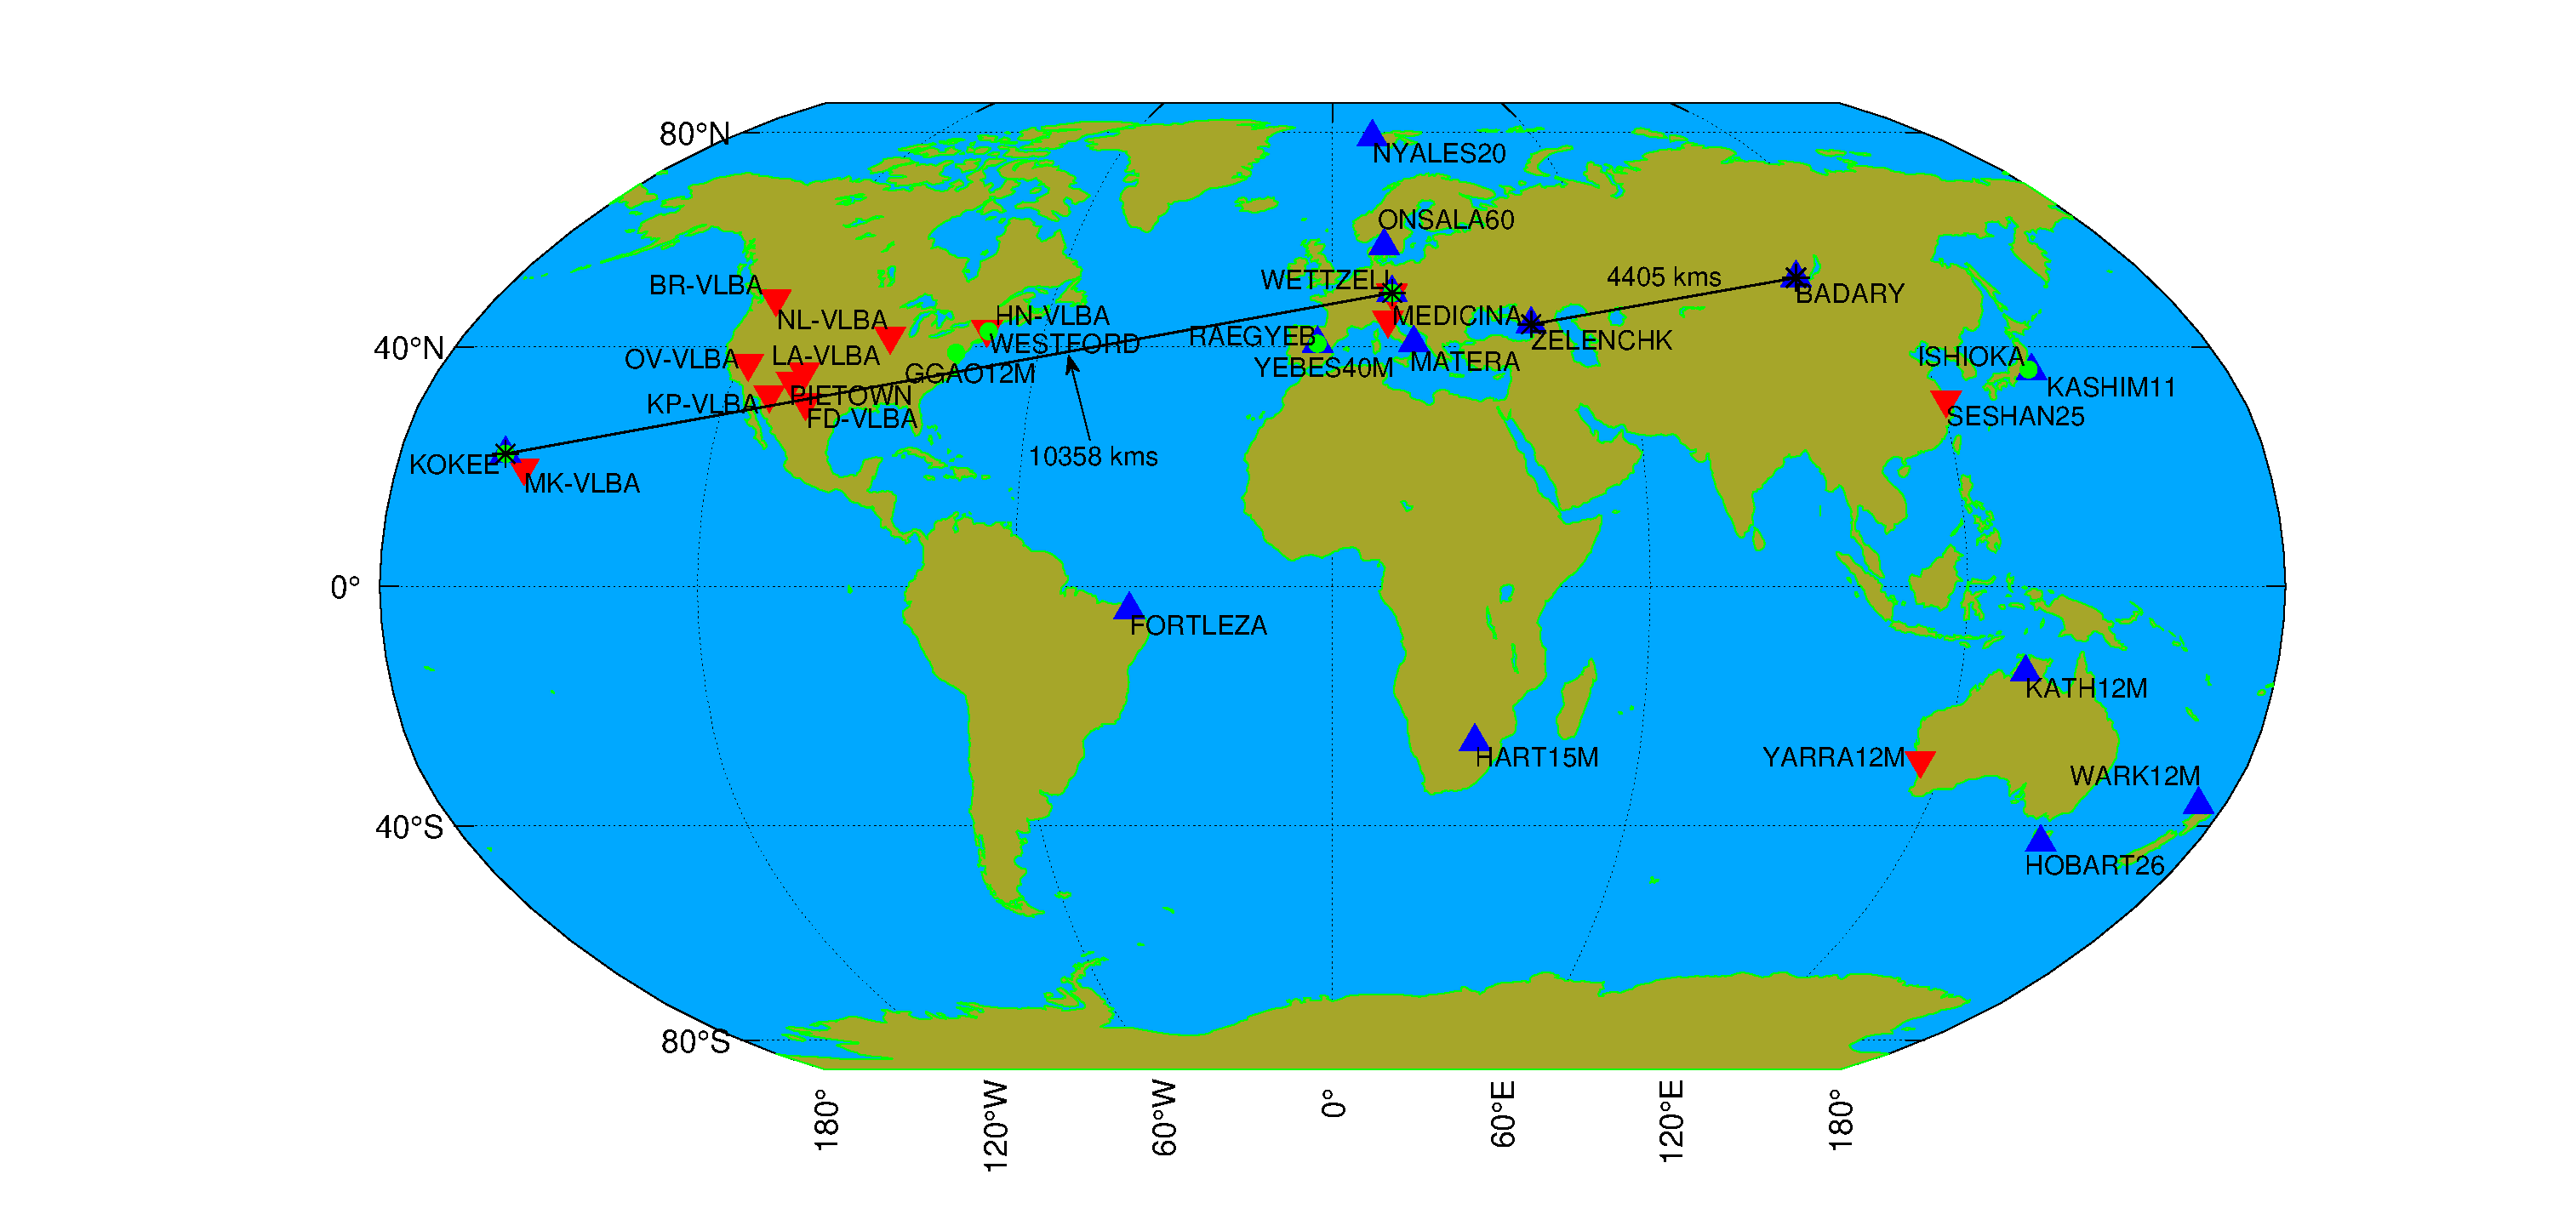
\includegraphics[scale=0.31]{VLBI_station_c.eps}
    \caption{Geographical representation of the stations of the various network. Legacy (S/X) stations in VLBA network (marked as the red triangle), IVS network (marked as the blue triangle); VGOS stations are represented by a Green circle; stations which participate in intensives are indicated by a black cross and their baselines are represented by a black solid line. \citep{rauteffect}}
    \label{fig:cont17stations}
\end{figure}

\begin{figure}[h]
    \centering
    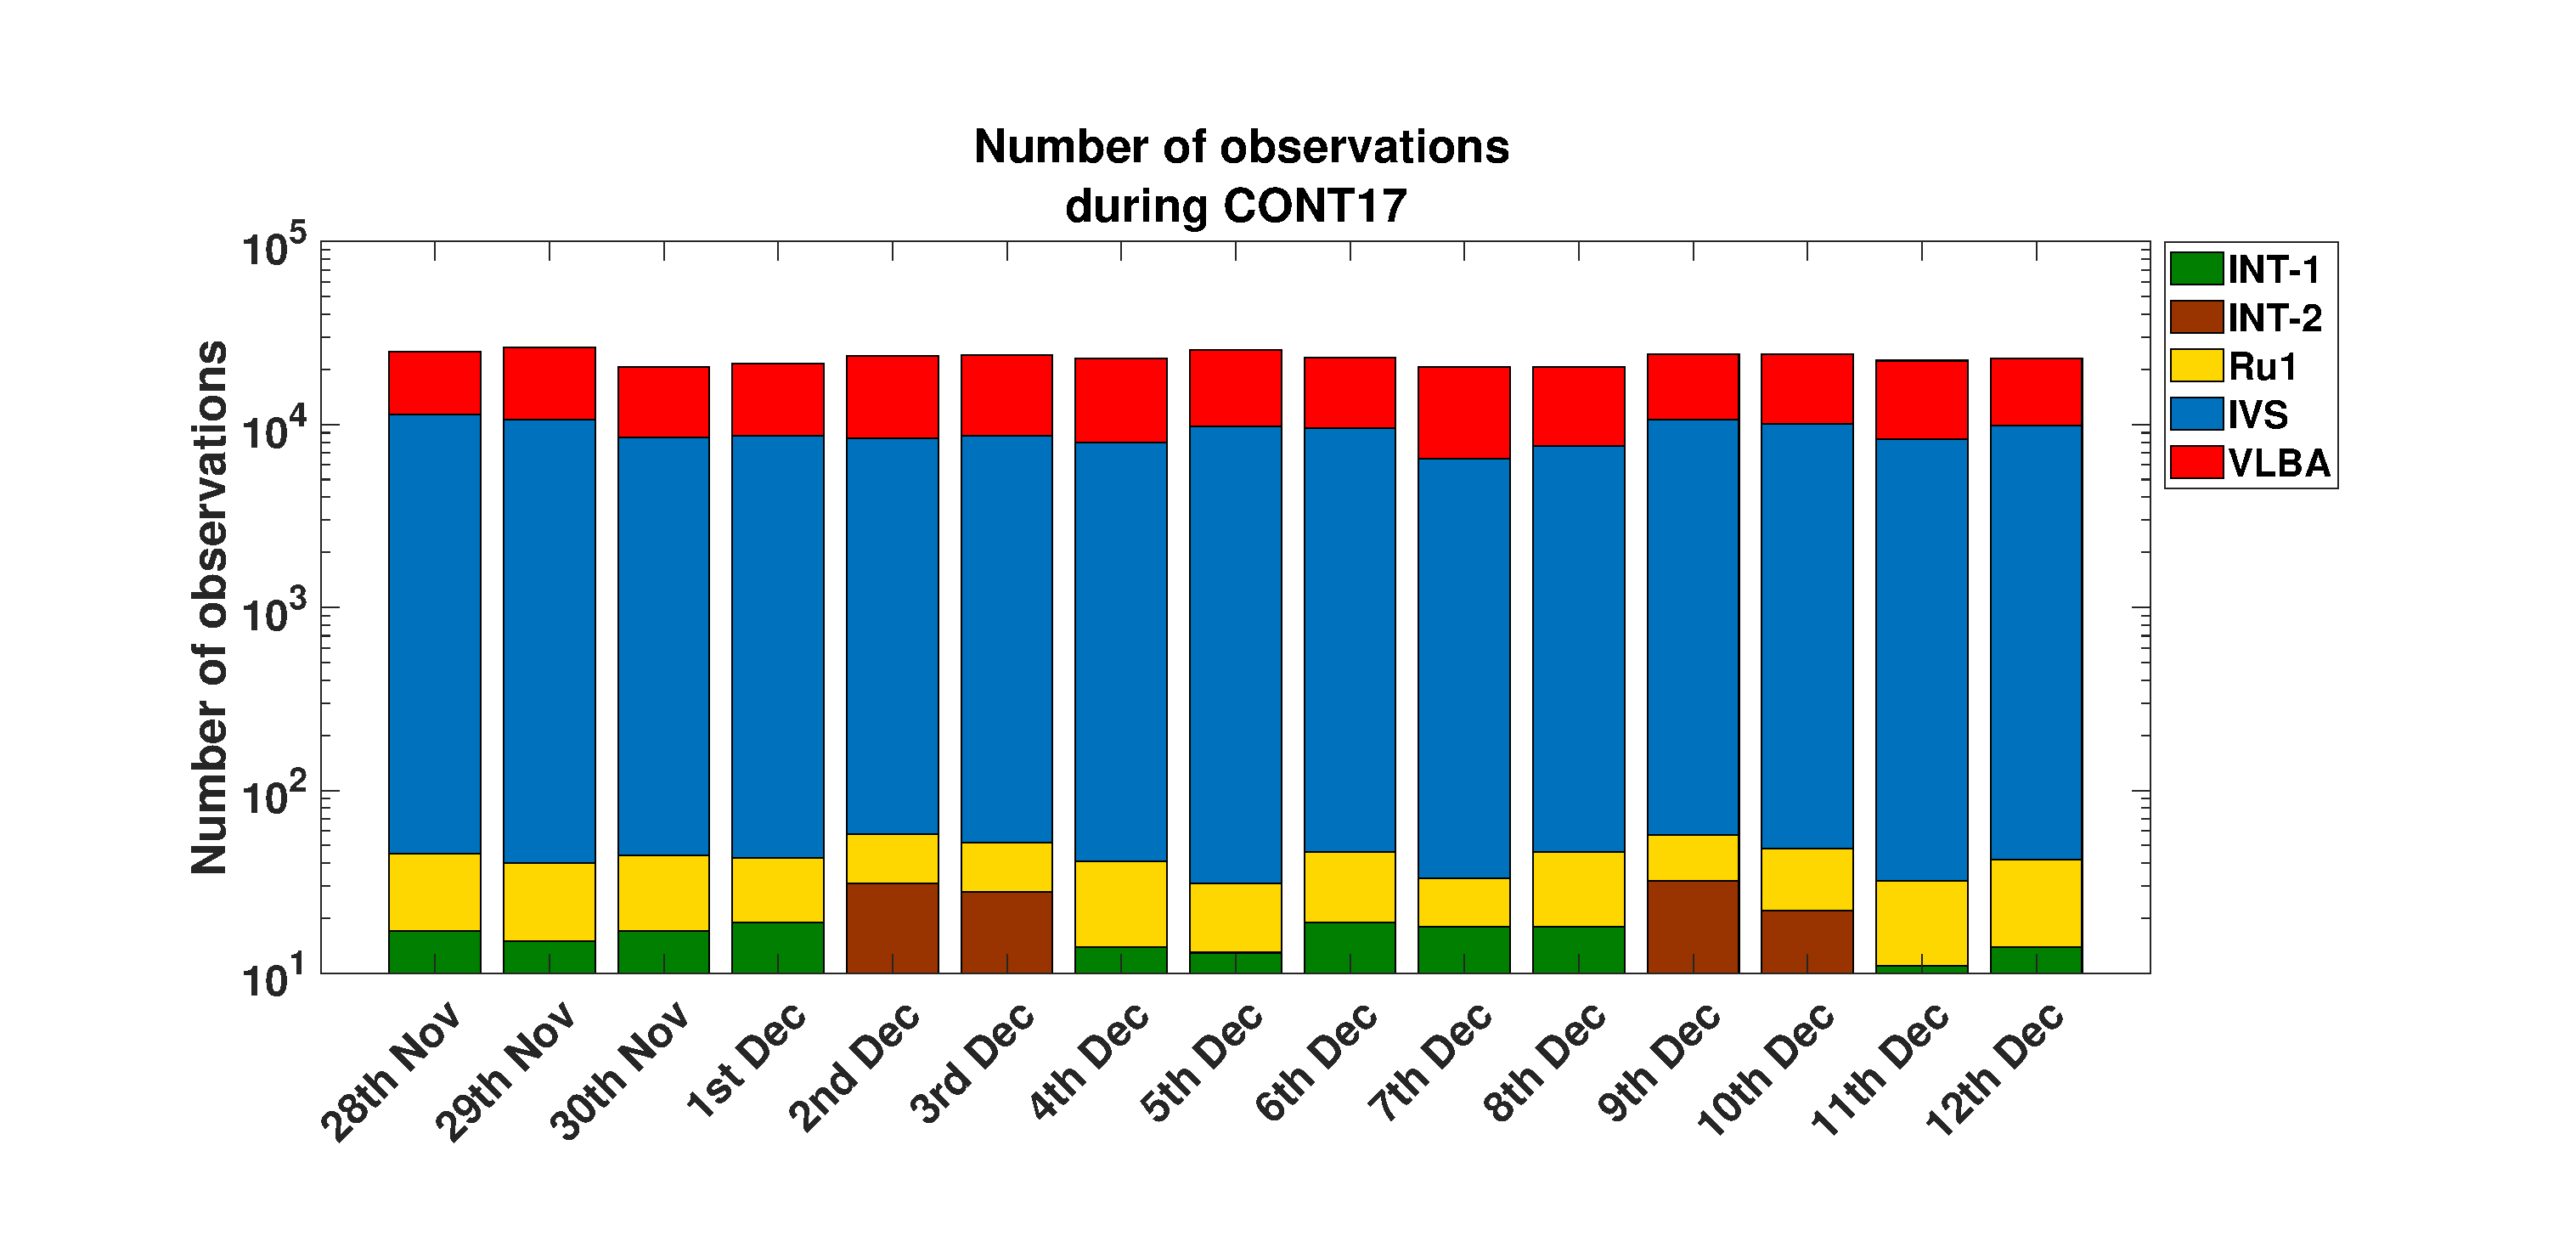
\includegraphics[scale=0.3]{noofobslog.eps}
    \caption{Number of VLBI observation during CONT17 campaign (observations from VGOS are not included). (\textit{y-axis has logarithmic scale})}
    \label{fig:noofobs}
\end{figure}

\begin{table}[h]
\centering
\caption{Overview of Intensives during CONT17.}
\label{tab:intstations}
\begin{tabular}{cccc}
\hline
  & \textbf{IVS-INT1} & \textbf{IVS-INT2} & \textbf{Ru1} \\ \hline
\textbf{Stations} & \begin{tabular}[c]{@{}l@{}}Wettzell (Germany)\\ Kokee Park (USA)\end{tabular} & \begin{tabular}[c]{@{}l@{}}Wettzell (Germany)\\ Kokee Park (USA\end{tabular} & \begin{tabular}[c]{@{}l@{}}Badary (Russia) \\ \\ Zelenchk (Russia)\end{tabular} \\ \hline
\textbf{Length of baseline (km)} & 10,357.4 & 10,357.4 & 4,405 \\
\textbf{East-West dimension (km)} & 10,072 & 10,072 & 4364.7 \\
\textbf{North-South dimension (km)} & 2,414 & 2,414 & 595.7 \\
\textbf{Observing days} & \begin{tabular}[c]{@{}l@{}}28th Nov - 1st Dec,\\ 4th - 8th Dec,\\ 11th -12th Dec\end{tabular} & \begin{tabular}[c]{@{}l@{}}2nd, 3rd, 9th, \\ \\ 10th Dec\end{tabular} & 28th Nov - 12th Dec \\
\textbf{Time frame of observations} & 18:30 - 19:30 & 07:30 - 08:30 & \begin{tabular}[c]{@{}l@{}}30th Nov, 4th \& 5th Dec: 19:30 - 20.30\\ 3rd \& 11th Dec: 20:30 - 21:30\\ Remaining days: 19:00 - 20:00\end{tabular} \\ \hline
\end{tabular}
\end{table}


\section{DATA ANALYSIS}
The dUT1 from CONT17 data was estimated with VieVs@GFZ(\citep{nilsson2015application}. For our analysis, the models and the apriori used are shown in the table~\ref{tab:models}. At first, the dUT1 estimated from IVS, VLBA, and combined legacy networks were compared. The dUT1 was estimated for one day and 1-hour temporal resolutions. Here the standard parameterization for a 24-hour session was used (see table~\ref{tab:param}). Secondly, dUT1 from intensives is estimated, where the standard parameterization for Intensives was followed (see table~\ref{tab:param}). These estimated dUT1 values are compared with dUT1 values estimated from the legacy networks.
\begin{table}[]
\caption{Standard parameterization used for analysing intensive and 24-hour VLBI sessions (*high relative constraint)}
\label{tab:param}
\centering
\begin{tabular}{|c|c|c|c|}
\hline
\multicolumn{2}{|c|}{\multirow{\textbf{Parameters}}} & \multicolumn{2}{c|}{\textbf{LSM parameterization}} \\ \cline{3-4} 
\multicolumn{2}{|c|}{} & \textbf{Intensives} & \textbf{24-hour} \\ \hline
\multirow{\textbf{\begin{tabular}[c]{@{}c@{}}Troposphere \\ \\ Estimation\end{tabular}}} & Zenith wet delays & Estimated & Estimated \\ \cline{2-4} 
 & North gradients & Not Estimated & Estimated \\ \cline{2-4} 
 & East gradients & Not Estimated & Estimated \\ \hline
\textbf{Clock Estimation} &  & Estimated & Estimated \\ \hline
\multirow{\textbf{EOP}} & x-pole & Not Estimated & Estimated \\ \cline{2-4} 
 & y-pole & Not Estimated & Estimated \\ \cline{2-4} 
 & UT1-UTC & Estimated* & Estimated \\ \cline{2-4} 
 & nutdx & Not Estimated & Estimated \\ \cline{2-4} 
 & nutdy & Not Estimated & Estimated \\ \hline
\textbf{Station Coordinates} &  & Not Estimated & Estimated \\ \hline
\textbf{Source Coordinates} &  & Not Estimated & Estimated \\ \hline
\end{tabular}
\end{table}

\begin{table}[]
\centering
\caption{A priori and correction models used for different parameters}
\label{tab:models}
\begin{tabular}{ccc}
\hline
\multicolumn{2}{c}{\textbf{Parameters}} & \textbf{Models/ Frames} \\ \Xhline{1pt}
\multirow{\textbf{Reference frames}} & Terrestial reference frame & ITRF2014 \\
 & Celestial reference frame & ICRF3 \\
\textbf{Ephimerides} & Ephimerides & JPL 421 \\
\multirow{\textbf{Troposphere}} & Pressure & GPT2 \\
 & Temperature & GPT2 \\
 & Mapping functions & Potsdam mapping function (PMF) \\
 & Gradients & APG (Bohm) \\
\textbf{Ionosphere} & Ionosphere delay & From NGS \\
\multirow{\textbf{Station models}} & Tidal Ocean loading & FES2004 \\
 & Tidal Atmosphere loading & vandam \\
 & Mean pole model & IERS 2015 \\
\multirow{\textbf{EOP}} & A priori time series & finals (Bulletin A) \\
 & Precession/Nutation model & IAU 2006/200A \\ \hline
\end{tabular}
\end{table}

\section{RESULTS}
\subsection{dUT1 from legacy CONT17 sessions}
The dUT1 time-series was estimated from 24-hour sessions of IVS, VLBA, and combined network (IVS + VLBA) using global solutions in VieVs@GFZ software. We also estimated dUT1 from intensive sessions from IVS-INT1, IVS-INT2 and Ru1 networks. The dUT1 were estimated for one day and one-hour resolution. \\
As we can see from the figure~\ref{fig:dut1d} that dUT1 estimated from the combined network has approximately average values of dUT1 estimated from individual legacy networks, for both resolutions. The dUT1 from combined networks also has smaller formal errors and fewer outliers. This can be explained as the combined network has significantly more observations and participating stations. The dUT1 estimated from combined and individual legacy networks are consistent with each other. The hourly dUT1 contains sub-daily variations which can be seen in the figure~\ref{fig:dut1hr}. However, the mean error of hourly dUT1 is significantly higher than the mean error of daily dUT1 as seen in the table~\ref{tab:rmsdut1}. The reason for this can be due to lesser number of observations per interval in the case of hourly resolution. \\
To understand the relationship between dUT1 estimated from IVS and VLBA network, we computed the correlation coefficient between them. For one day resolution, the correlation was found to be 0.93 and for one-hour resolution, it is 0.61. The decrease in correlation coefficient for hourly resolution might be due to different amount of sub-daily variations in the IVS and VLBA network. \\
\begin{figure}[h]
    \centering
    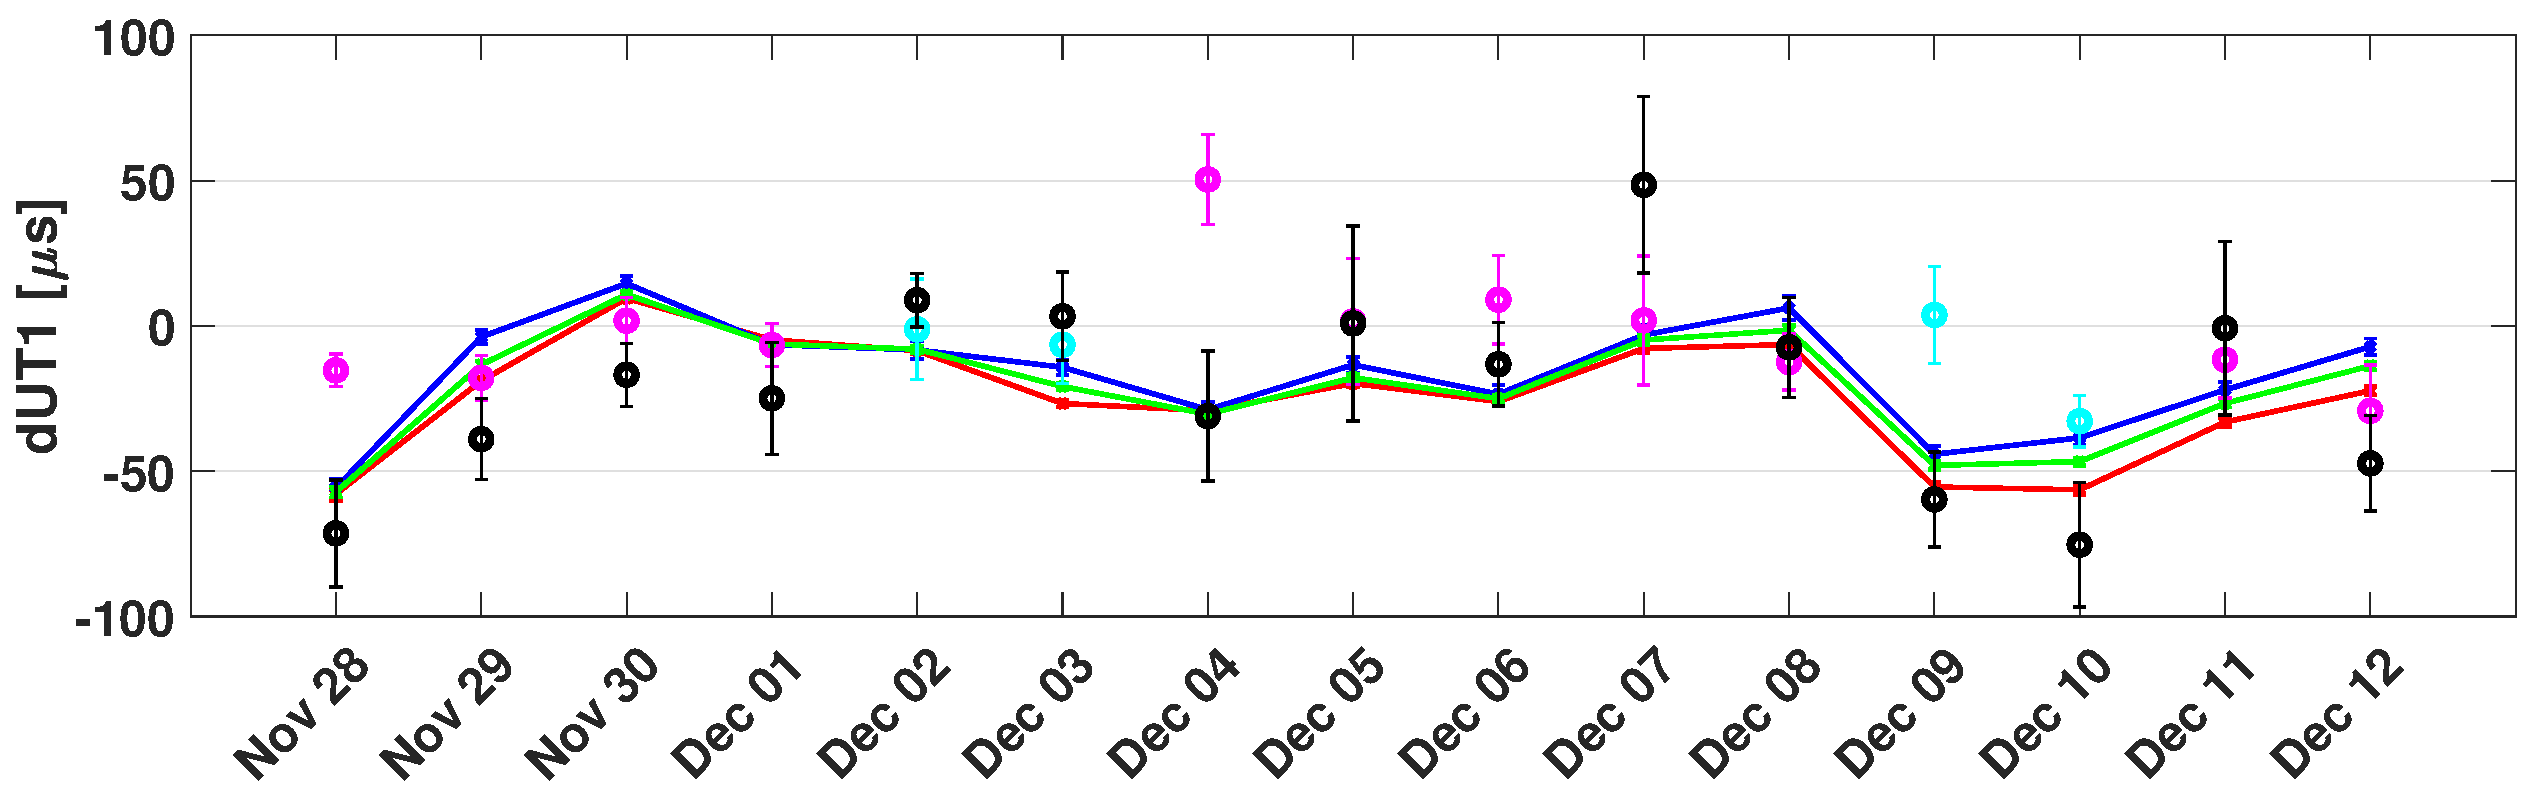
\includegraphics[scale=0.3]{dut11dayint.eps}
    \caption{dUT1 estimates for 1 day resolution; The blue, red and green line represents dUT1 estimated from IVS, VLBA and combined network, respectively. The magenta, cyan and black circle represents dUT1 from IVS-INT1, IVS-INT2, and Ru1 intensive networks, respectively.}
    \label{fig:dut1d}
\end{figure}
\begin{figure}[h]
    \centering
    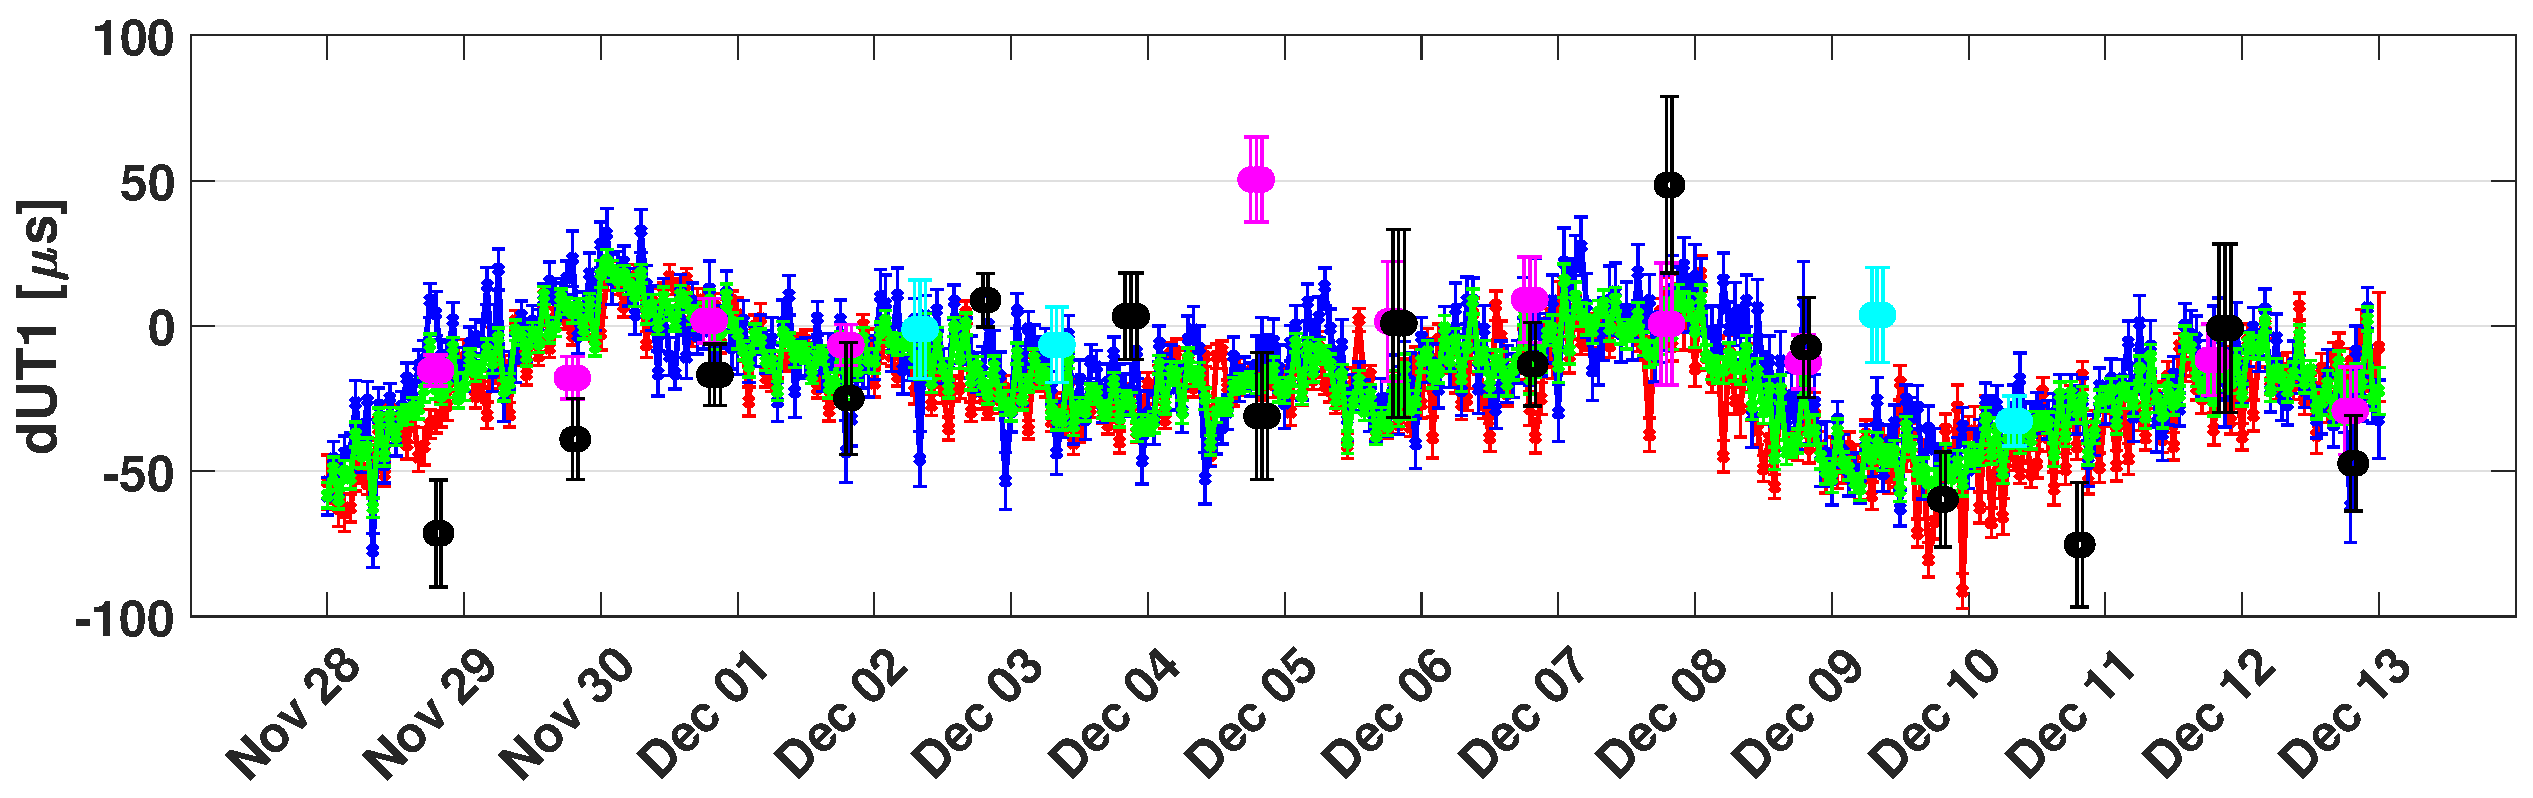
\includegraphics[scale=0.3]{dut11hrint.eps}
    \caption{dUT1 estimates for 1 day (top) and 1-hour (below) resolution; The blue, red and green line represents dUT1 estimated from IVS, VLBA and combined network, respectively. The magenta, cyan and black circle represents dUT1 from IVS-INT1, IVS-INT2, and Ru1 intensive networks, respectively.}
    \label{fig:dut1hr}
\end{figure}
\begin{table}
\centering
\caption{WRMS values of the dUT1 from legacy and intensive networks and their corresponding mean errors. 
(given values are in $\mu secs$)}
\label{tab:rmsdut1}
\begin{tabular}{ccccc}
\hline
Networks & \multicolumn{2}{c}{1 day} & \multicolumn{2}{c}{1 hour} \\ \hline
(in $\mu secs$) & \begin{tabular}[c]{@{}c@{}}WRMS\end{tabular} & \begin{tabular}[c]{@{}c@{}}Mean\\ Error\end{tabular} & \begin{tabular}[c]{@{}c@{}}WRMS\end{tabular} & \begin{tabular}[c]{@{}c@{}}Mean\\ Error\end{tabular} \\ \Xhline{1.2}
IVS & 27.09 & 2.97 & 23.57 & 7.63 \\
VLBA & 25.96 & 1.62 & 26.16 & 4.48 \\
Combined & 26.21 & 1.47 & 25.55 & 3.76 \\ \hdashline
IVS-INT & 17.71 & 13.20 & 17.75 & 12.61 \\
Ru1 & 34.01 & 19.25 & 32.10 & 19.42 \\ \hline
\end{tabular}
\end{table}

\subsection{dUT1 from Intensive sessions}
The dUT1 are estimated from the three different intensive networks i.e., IVS-INT1, IVS-INT2, and Ru1. We can observe that dUT1 estimated from Russian intensives have higher formal errors as compared to IVS intensives (see table~\ref{tab:rmsdut1}). The main reason for this is due to the different baseline length, and dUT1 is sensitive to a more extended east-west baseline. Since Russian intensive (4405 km) has a shorter baseline than IVS intensive(10358 km), resulting in higher formal errors in dUT1. \\
Now we will compare dUT1 values from intensive sessions with dUT1 estimated from 24-hour legacy networks. The daily dUT1 values from the 3 intensive networks are over-plotted with dUT1 from IVS, VLBA and combined networks (see figure~\ref{fig:dut1d}). Similar over-plot is generated for hourly resolution (see figure~\ref{fig:dut1hr}).
It can be observed from the figure~\ref{fig:dut1d}, that most of the dUT1 from IVS intensives and some dUT1 from Russian intensives show good agreement with the dUT1 from 24-hour sessions. However, the formals errors are significantly higher in dUT1 from intensives. The possible reason regarding the inconsistencies in dUT1 can be explained as most parameters are not estimated, i.e., fixed to a priori values when estimating dUT1 from intensives. The inaccuracies present in the a priori values of the fixed parameters, it will further propagate in the dUT1 determination. To further validate the relationship between them, the correlation coefficient is computed. The coefficient between IVS intensives and IVS and VLBA networks is 0.10 and 0.28, respectively which is a low positive correlation between them. This could be due to different observing times of IVS-INT1 (evening) and IVS-INT2 (morning), it might have resulted in inconsistent dUT1 values. However, the correlation coefficient between Russian intensives with dUT1 from IVS, and VLBA network are approximately 0.70 , which considerably shows better agreement between them.  \\
In addition to the reason mentioned above, the inconsistencies between the dUT1 values could be present due to the different observing times. The estimated daily values of dUT1 from intensive sessions are computed from observations that span approximately one hour during a day, the sub-daily variations in dUT1 might be present in it. The sub-daily variations in daily dUT1 from legacy networks are not present as these variations are averaged out in such 24-hour sessions. This might be another possible reason for the inconsistencies present between the dUT1 estimated from intensives and legacy networks. To improve the agreement between them, we can compare the dUT1 values for the same interval. \\

This comparison can be done with two approaches. The first approach is to estimate the dUT1 from 24-hour sessions for an hourly resolution. Then we can compare dUT1 from the intensive session with the hourly dUT1 estimated from legacy networks for the corresponding interval when the intensive session took place. The other approach is to compute the dUT1 value from the intensive session and then extrapolate this value to the nearest midnight epoch (i.e., 00:00:00 UTC) using high-frequency EOP models. This dUT1 value can be compared to the daily dUT1 value estimated from the legacy networks. \\
In the first approach, we compare the hourly dUT1 estimated from the intensive sessions with corresponding intervals of hourly dUT1 estimated from IVS and VLBA network. For example, if the intensive session spans from 18:30 to 19:30, we get dUT1 for 18:00, 19:00, and 20:00 epoch. These dUT1 values should not vary due to high relative constraints applied while analyzing an intensive session. For better understanding, we calculated the WRMS differences between dUT1 estimated from intensives and 24-hour sessions. We plotted these values in figure~\ref{fig:wrmsdut1}.
The WRMS difference between daily dUT1 from intensive sessions and 24-hour sessions are kept as a reference value.
The dUT1 from IVS intensives show 46$\%$ more agreement with hourly dUT1 from IVS sessions and 5$\%$ less agreement with hourly dUT1 from VLBA sessions (see figure~\ref{fig:wrmsdut1}(a)). Whereas, dUT1 from Russian intensives show 34$\%$ less agreement with hourly dUT1 from IVS sessions and 30$\%$ more agreement with hourly dUT1 from VLBA sessions (see figure~\ref{fig:wrmsdut1}(b)). 
\begin{figure}[h]
    \centering
    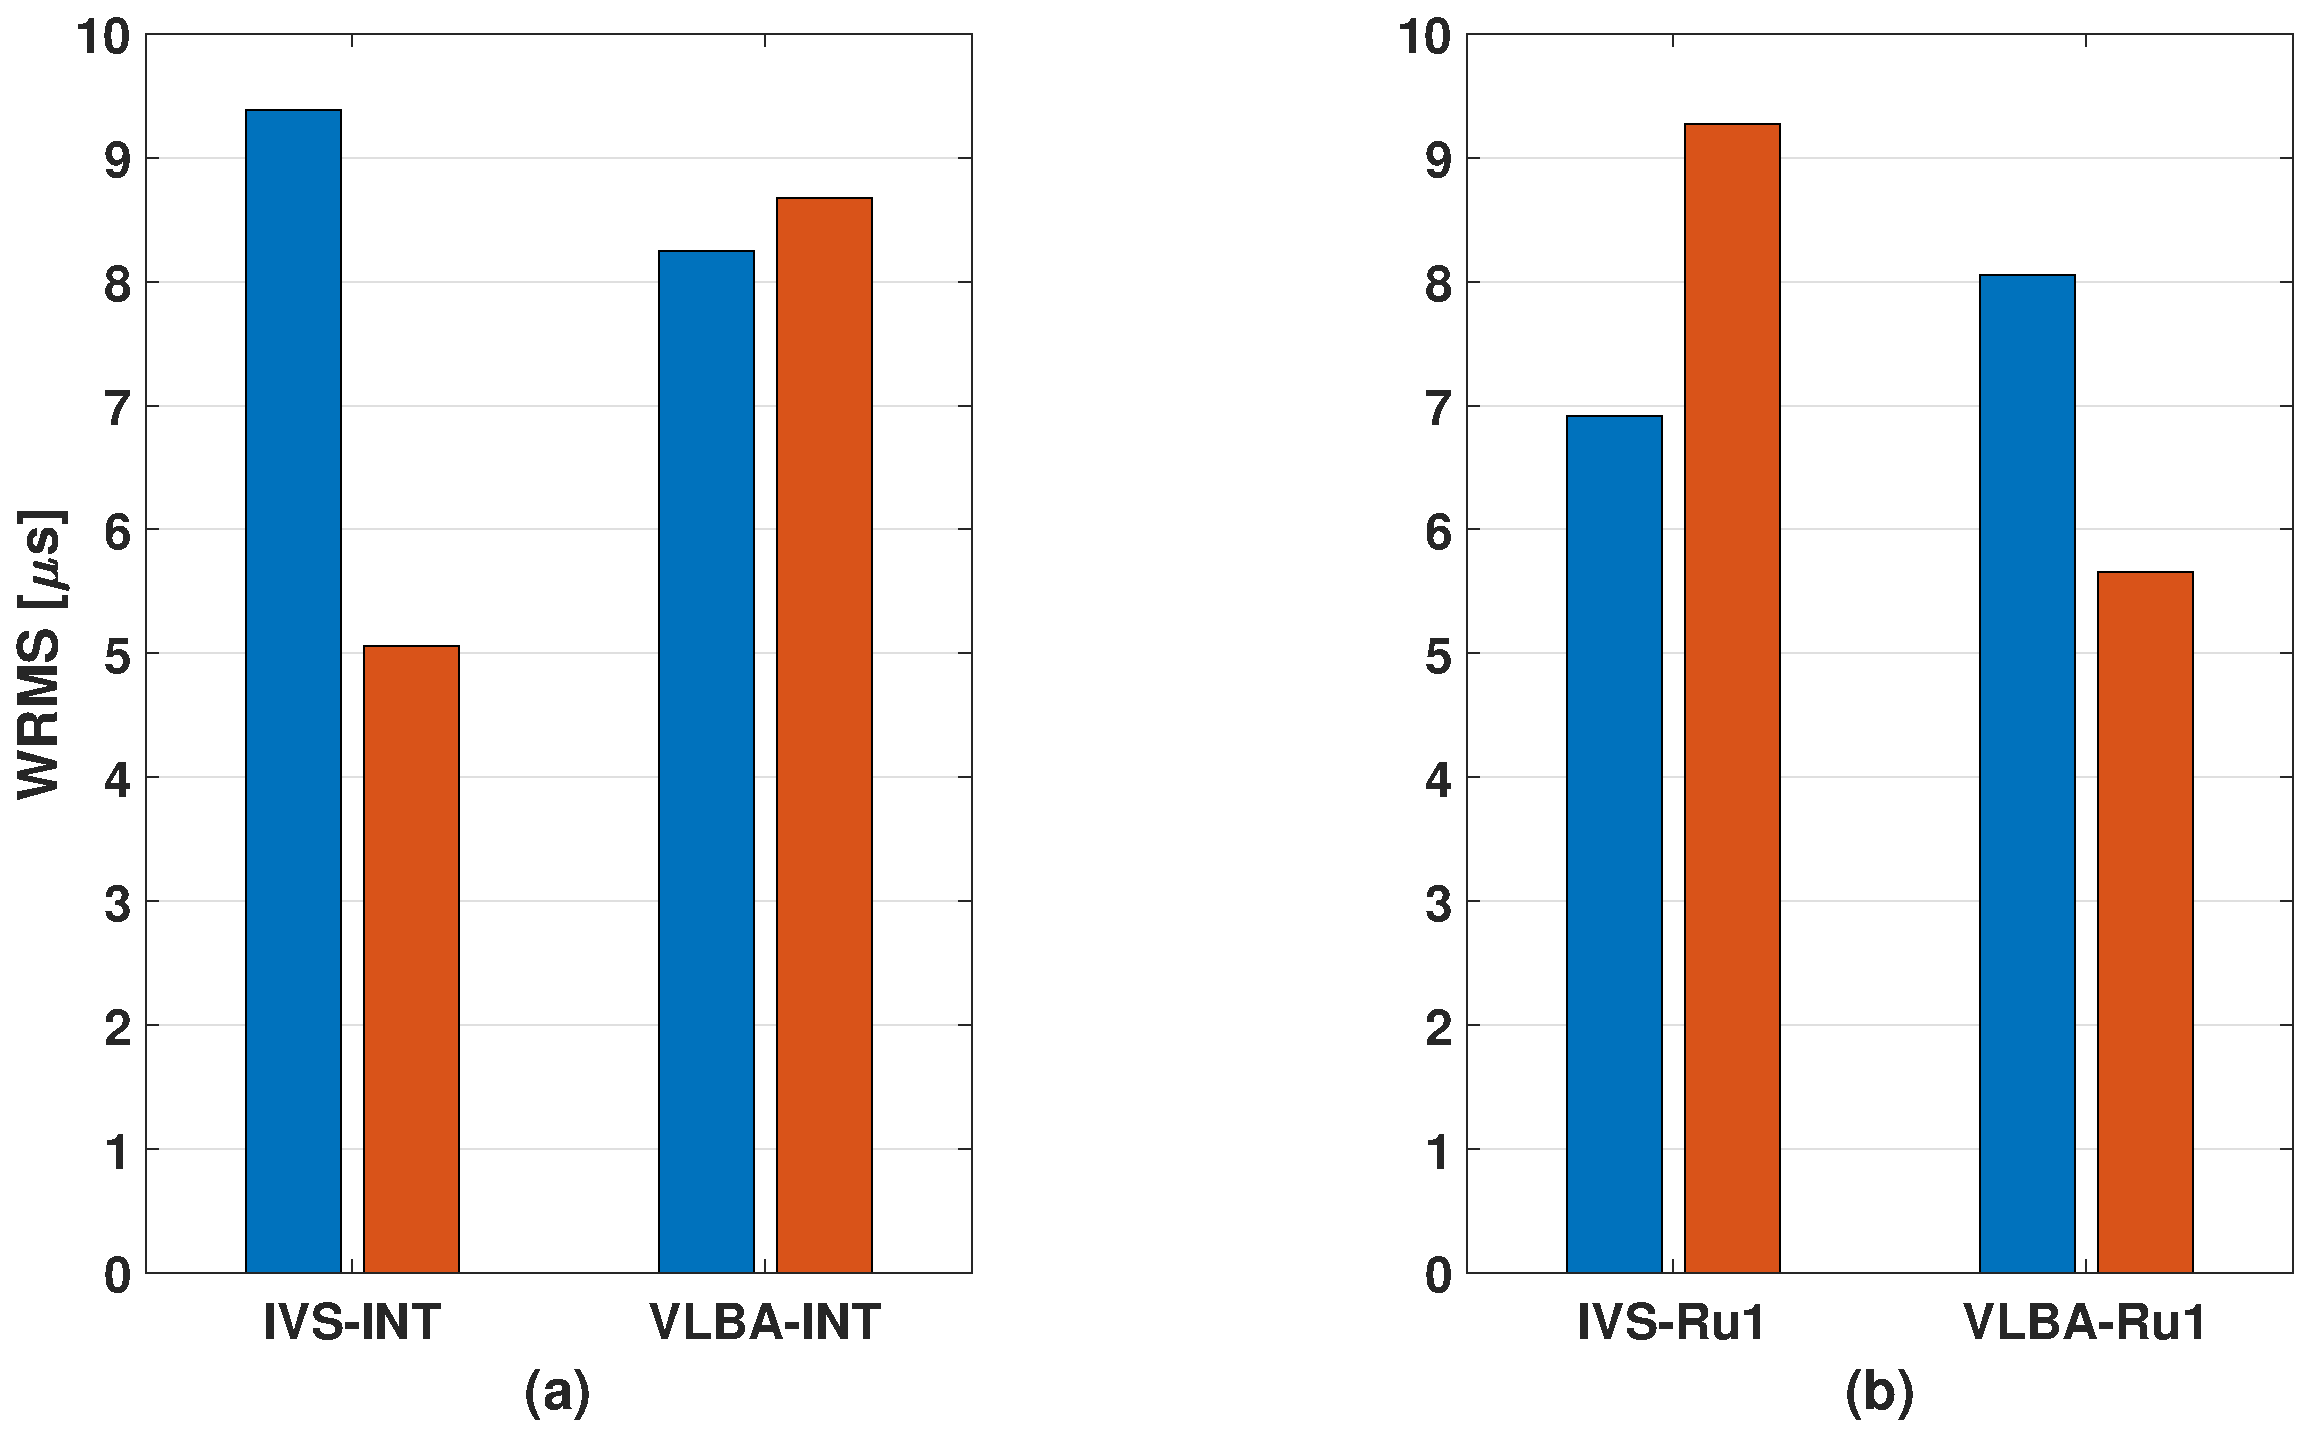
\includegraphics[scale=0.25]{wrmsdut1.eps}
    \caption{(a) WRMS difference between dUT1 time series estimated from IVS and VLBA network with INT intensive networks; (b) WRMS difference between dUT1 time series estimated from IVS and VLBA network with Russian intensive networks; \textit{Blue and red coloured bar represents difference in dUT1 for daily and hourly resolution, respectively.}
   }
    \label{fig:wrmsdut1}
\end{figure}
\subsection{Deriving dUT1 using high-frequency EOP models}
In this section, we have used HFEOP models as apriori values for estimating dUT1 from the intensive sessions. The HFEOP models used for the analysis are IERS 2010 model \citep{petit2010iers}, Desai model \citep{desai2016evaluating} and Gipson model \citep{gipson2015new}. The IERS 2010 and Desai model are based on ocean tide models whereas the Gipson model is empirically derived from 35 years of VLBI data. The reason for choosing the mentioned models (apart from IERS 2010 model) is that they perform better as compared to other HFEOP models according to \cite{nilsson2018evaluation}. We estimate dUT1 from the Intensives, keeping the beforehand mentioned HFEOP models as apriori and compare them with daily dUT1 from IVS and VLBA sessions. As there are small differences between the dUT1 from intensives using different hfeop models, we plotted the differences in WRMS of dUT1 from different hfeop w.r.t. IVS and VLBA network (see figure~\ref{fig:hfeopdut1}). \\
The difference in WRMS of dUT1 from intensives (without applying HFEOP) and legacy network are kept as reference. The dUT1 from intensives (INT) on applying Desai model shows improvement of 4.2$\%$ and 4.75$\%$ w.r.t. to IVS and VLBA, respectively (see figure~\ref{fig:hfeopdut1}(a)). Whereas, the dUT1 from Russian intensives on applying IERS 2010 model shows a marginal improvement of approx. 0.4$\%$ w.r.t. to dUT1 from IVS and VLBA network (see figure~\ref{fig:hfeopdut1}(b)). It can be observed that applying HFEOP model for deriving dUT1 from Russian intensive do not have a significant effect.
\begin{figure}[h]
    \centering
    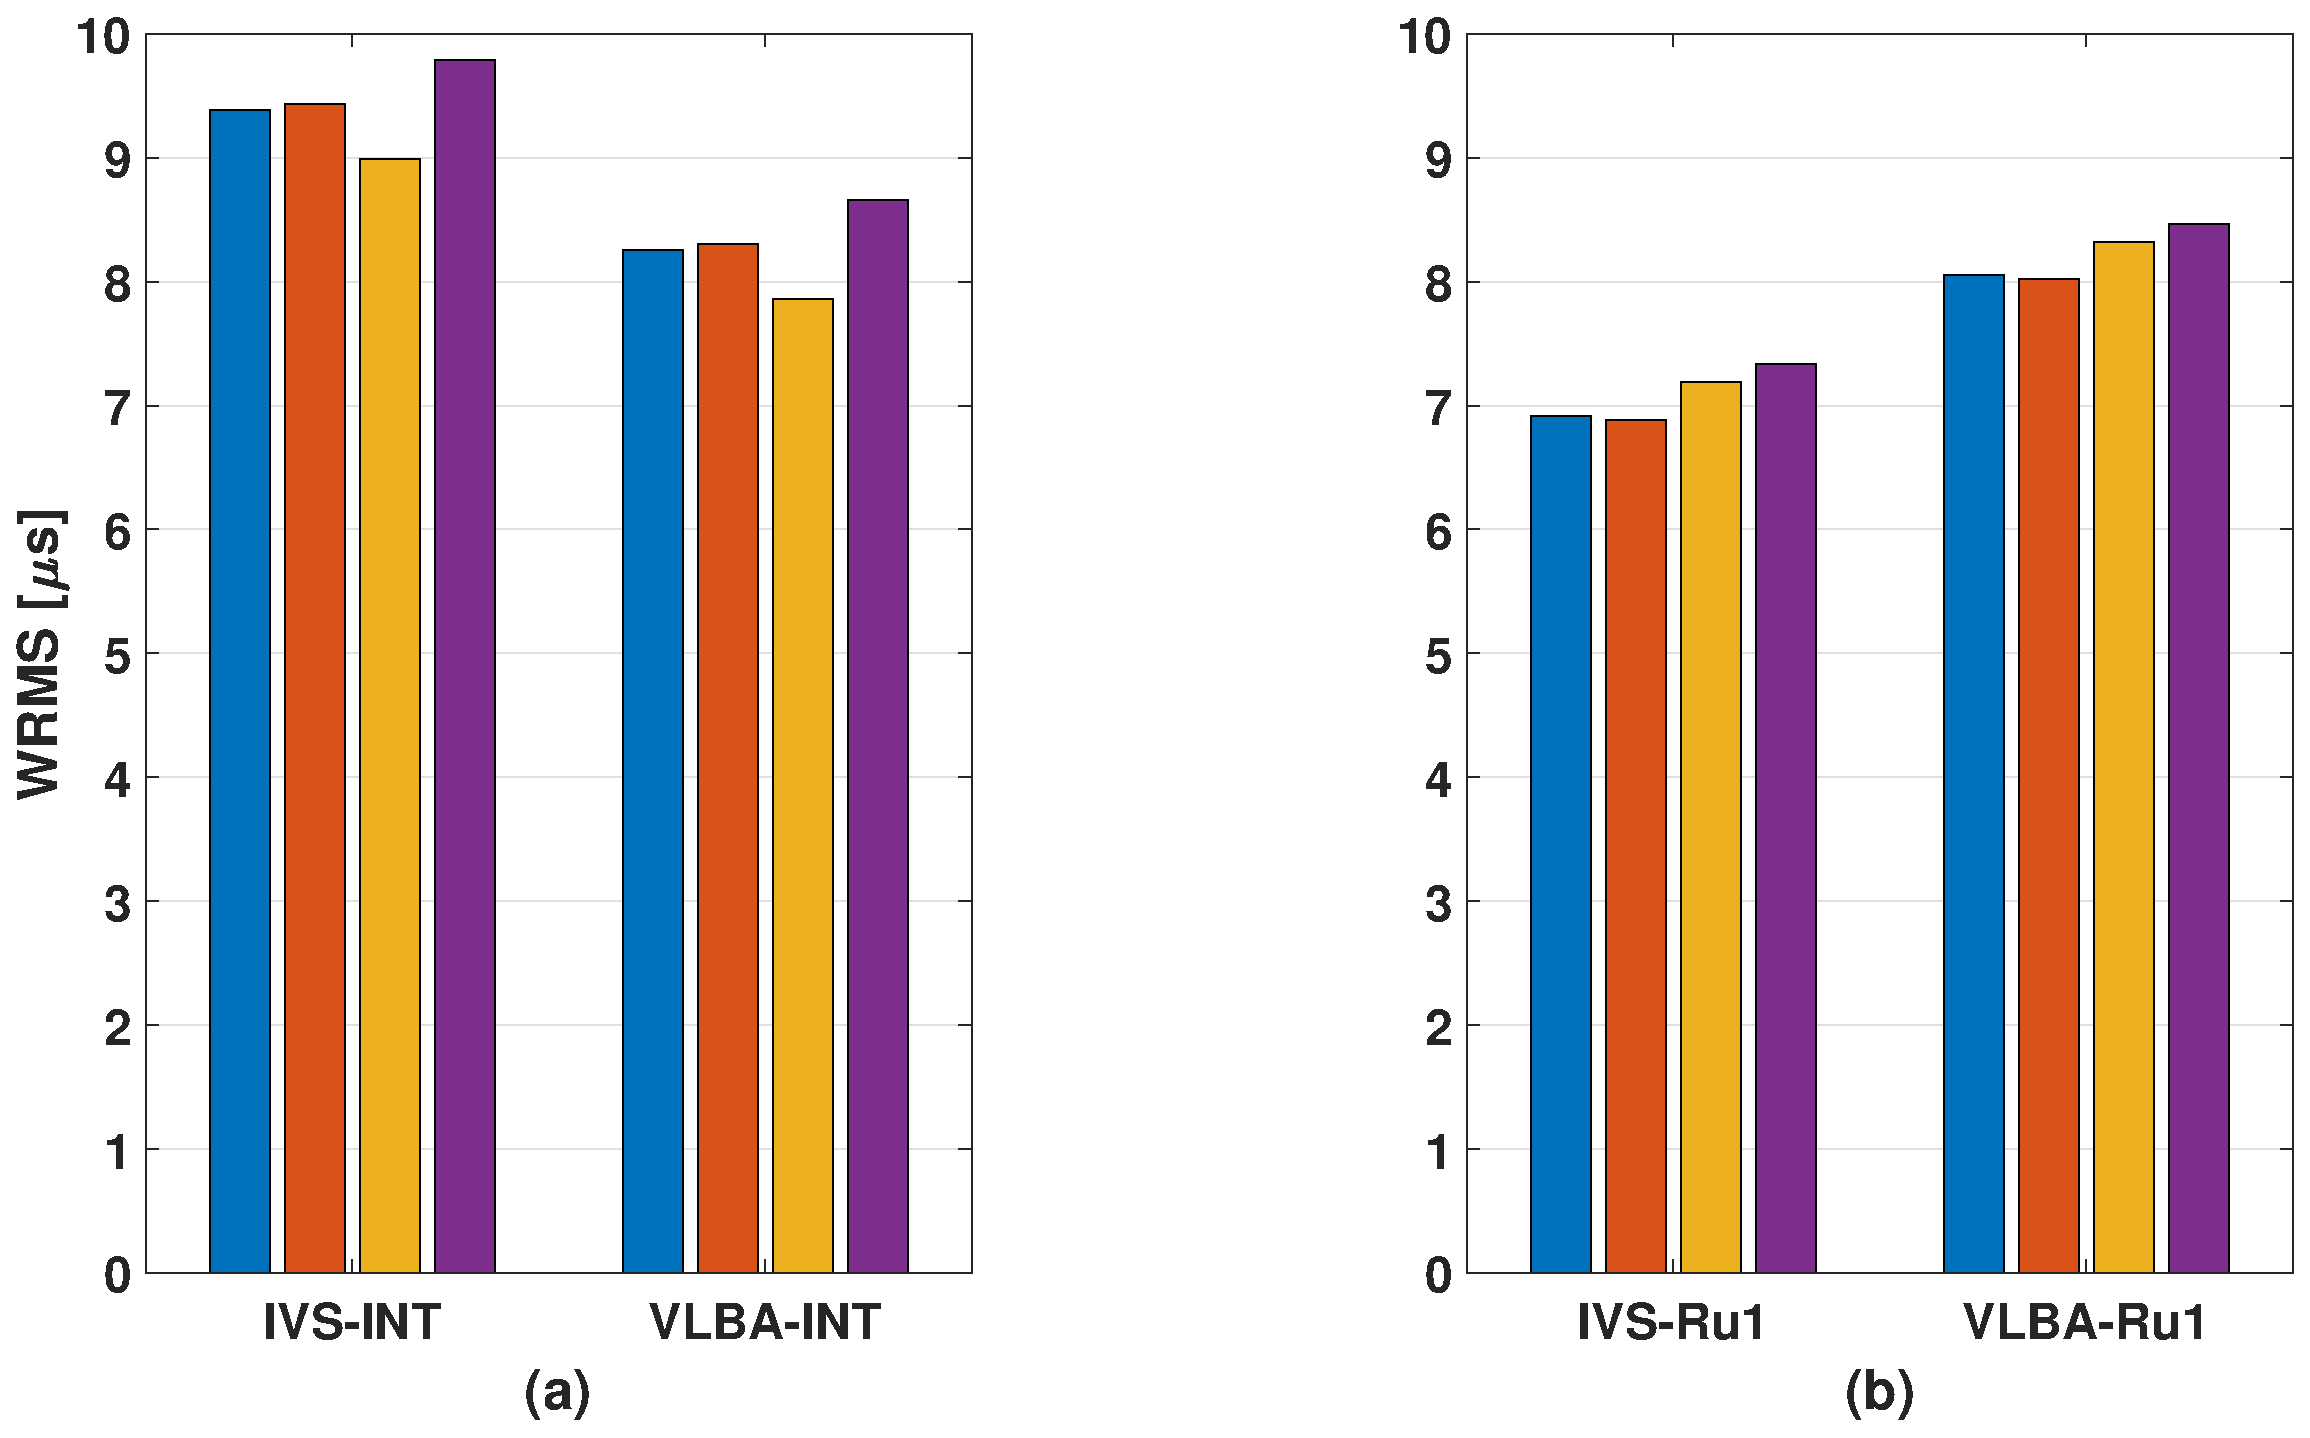
\includegraphics[scale=0.3]{wrmsdut1hfeop.eps}
    \caption{(a) WRMS difference between the dUT1 time series from INT intensives (applying HFEOP models) and IVS, and VLBA network; (b) WRMS difference between the dUT1 time series from Russian intensives (applying HFEOP models) and IVS, and VLBA network; \textit{Blue color represents that no HFEOP model was applied while estimating dUT1 from intensives. Red, yellow, and purple color represents that IERS 2010, Desai, and Gipson HFEOP was applied while estimating dUT1 from intensives.}}
    \label{fig:hfeopdut1}
\end{figure}
\section{CONCLUSIONS}
The dUT1 estimated from the VLBA network has more impact on the dUT1 from the combined network as VLBA contains several long east-west baselines. The correlation coefficient between daily dUT1 from two networks was highly positive whereas the coefficient between hourly dUT1 from 2 networks decreased by approx. 35$\%$. The possible reason for the reduction in correlation might be due to the different amount of sub-daily variations in the 2 networks. The hourly dUT1 showed higher formal errors compared to their daily dUT1 counterparts. Overall, dUT1 from the two networks gave similar results. We estimated dUT1 from IVS and Russian intensives. As the Russian baseline has a shorter baseline than IVS intensive baseline, it resulted in higher formal errors.\\
It has been observed that dUT1 from IVS intensives showed 46$\%$ more agreement with hourly dUT1 from IVS network and dUT1 from Russian intensive showed 30$\%$ more agreement with hourly dUT1 from VLBA network, this comparison was done w.r.t daily dUT1 values from legacy networks.\\
We applied HFEOP models while estimating from intensive sessions. An improvement of 4.2$\%$ and 4.75$\%$ w.r.t. IVS and VLBA network was seen when the Desai model was applied while analyzing IVS intensives as compared to when no HFEOP model was applied. However, no improvement was seen while analysing Russian intensives. \\
Concerning the future work, more rigorous analysis must be carried out to compare the results to further improve dUT1 estimation from intensive sessions. Further, if the intensive session took place close to midnight, it is possible to obtain dUT1 value having more agreement with dUT1 from 24-hour session. In this way, the effect of the sub-daily variations in dUT1 estimated from intensives would decrease. Secondly, HFEOP model such as Desai model can be applied while estimating dUT1 from intensives, however more work needs to be done in that area. 

%\begin{acknowledgements}
%If you'd like to thank anyone, place your comments here
%and remove the percent signs.
%\end{acknowledgements}

% BibTeX users please use one of
% \bibliographystyle{spbasic}      % basic style, author-year citations
% %\bibliographystyle{spmpsci}      % mathematics and physical sciences
% %\bibliographystyle{spphys}       % APS-like style for physics
% %\bibliography{}   % name your BibTeX data base

% % Non-BibTeX users please use
% \begin{thebibliography}{}
% %
% % and use \bibitem to create references. Consult the Instructions
% % for authors for reference list style.
% %
% \bibitem{RefJ}
% % Format for Journal Reference
% Author, Article title, Journal, Volume, page numbers (year)
% % Format for books
% \bibitem{RefB}
% Author, Book title, page numbers. Publisher, place (year)
% % etc
% \end{thebibliography}
\bibliography{reference}
\bibliographystyle{spbasic}
\end{document}
% end of file template.tex